%%%%%%%%%%%%%%%%%%%%%%%%%%%%%%%%%%%%%%%%%
% Texas A&M University Physics Template
% This template has been downloaded from:
% http://www.LaTeXTemplates.com
%
% Modified by Joe Becker
%
% License:
% CC BY-NC-SA 3.0 (http://creativecommons.org/licenses/by-nc-sa/3.0/)
%
%%%%%%%%%%%%%%%%%%%%%%%%%%%%%%%%%%%%%%%%%

%----------------------------------------------------------------------------------------
%	PACKAGES AND THEMES
%----------------------------------------------------------------------------------------

\documentclass{beamer}

\mode<presentation> 

\usetheme{Madrid}
\usecolortheme{dolphin}
\usefonttheme{professionalfonts}

\setbeamertemplate{navigation symbols}{} 

\setbeamertemplate{footline}
{
\leavevmode%
\hbox{%
    \begin{beamercolorbox}[wd=.333333\paperwidth,ht=2.25ex,dp=1ex,center]{section in head/foot}%
        \usebeamerfont{author in head/foot}\insertshortauthor \ {(\insertshortinstitute)}
    \end{beamercolorbox}%
    \begin{beamercolorbox}[wd=.333333\paperwidth,ht=2.25ex,dp=1ex,center]{section in head/foot}%
        \usebeamerfont{title in head/foot}\insertshorttitle
    \end{beamercolorbox}%
    \begin{beamercolorbox}[wd=.333333\paperwidth,ht=2.25ex,dp=1ex,right]{section in head/foot}%
        \usebeamerfont{date in head/foot}\insertshortdate{}\hspace*{2em}
    \end{beamercolorbox}}%
    \vskip0pt%
}

\setbeamertemplate{frametitle}
{
    \begin{beamercolorbox}[sep=0.3cm,ht=1.8em,wd=\paperwidth]{frametitle}
        \vbox{}\vskip-0.0ex%
        \strut\insertframetitle\strut
        \hfill
        
\includegraphics[height=1.8em,keepaspectratio]{Images/TAMU_logo_box.png}
        \vskip-2.8ex%
    \end{beamercolorbox}
}

\definecolor{maroon}{RGB}{80,0,0}

\setbeamercolor{title}{bg=maroon, fg=white}
\setbeamercolor{block title}{bg=maroon, fg=white}
\setbeamercolor{block body}{bg=maroon!05, fg=black}
\setbeamercolor{frametitle}{fg=maroon, bg=white}
\setbeamercolor{item}{fg=maroon}
\setbeamercolor{section in head/foot}{bg=maroon, fg=white}


\usepackage{graphicx}
\usepackage{booktabs}
\usepackage{textpos} 
\usepackage{media9}


%----------------------------------------------------------------------------------------
%	TITLE PAGE
%----------------------------------------------------------------------------------------

\title[]{Nitrogen-Vacancy Photoionization from the Singlet State: Micro-diamond electrodes}

\author[J. Becker]{Joe Becker}

\institute[Texas A\&M]{Texas A\&M Department of Physics and Astronomy

\medskip
\textit{jbecker@physics.tamu.edu} 
}

\date{October 28, 2016} 

\titlegraphic{
\includegraphics[height=1.5cm]{Images/TAMU_logo.png}}

%----------------------------------------------------------------------------------------
% PRESENTATION SLIDES
%----------------------------------------------------------------------------------------

\begin{document}
\setbeamertemplate{items}[circle]

\begin{frame}
\titlepage 
\end{frame}

\section{Background}
\begin{frame}\frametitle{Nitrogen-Vacancy Diamonds}
    \begin{block}{NV Defect}
        \centering
        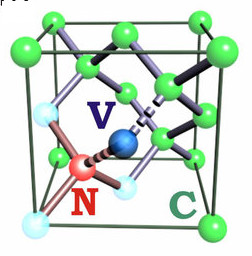
\includegraphics[width=0.55\textwidth]{Images/NVDiamond.jpg}

        I. V. Fedotov, et al.  Sci. Rep. 4, 5362 (2014).
    \end{block}
\end{frame}

\begin{frame}\frametitle{Nitrogen-Vacancy Photoionization}
    \begin{block}{NV Energy and Fluorescence}
        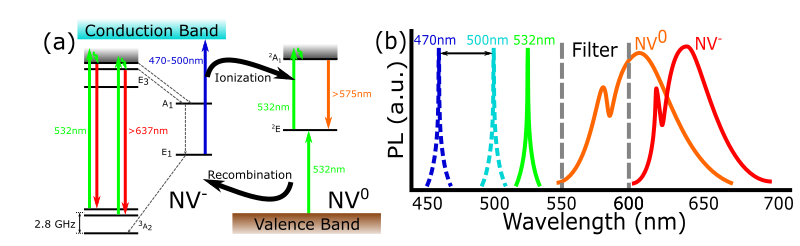
\includegraphics[width=1.0\textwidth]{Images/IonizationEnergyandFilter.png}
    \end{block}
\end{frame}

\begin{frame}\frametitle{Two Photon Photoionization}
    \centering
    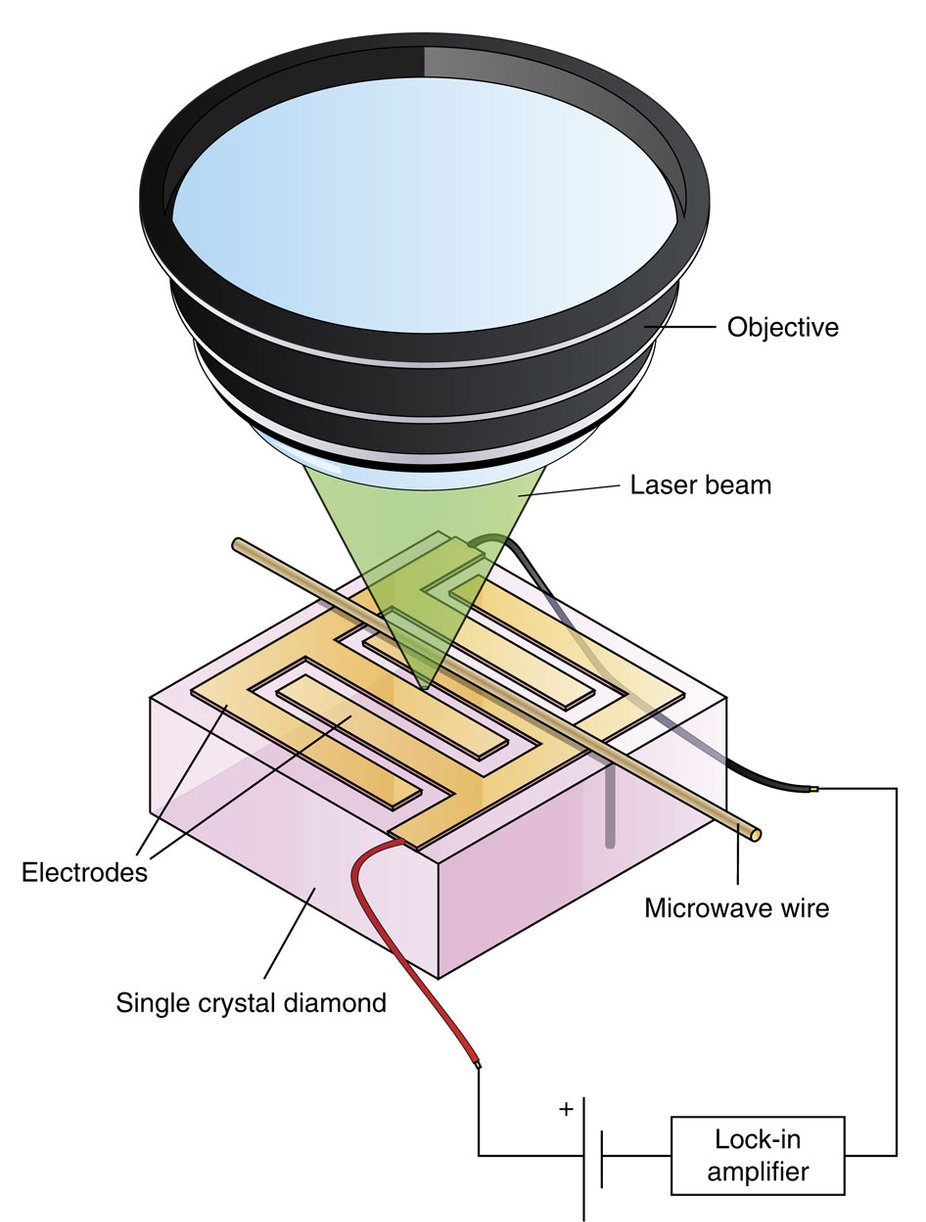
\includegraphics[width=0.45\textwidth]{Images/TwoPhotonGroup.png}
    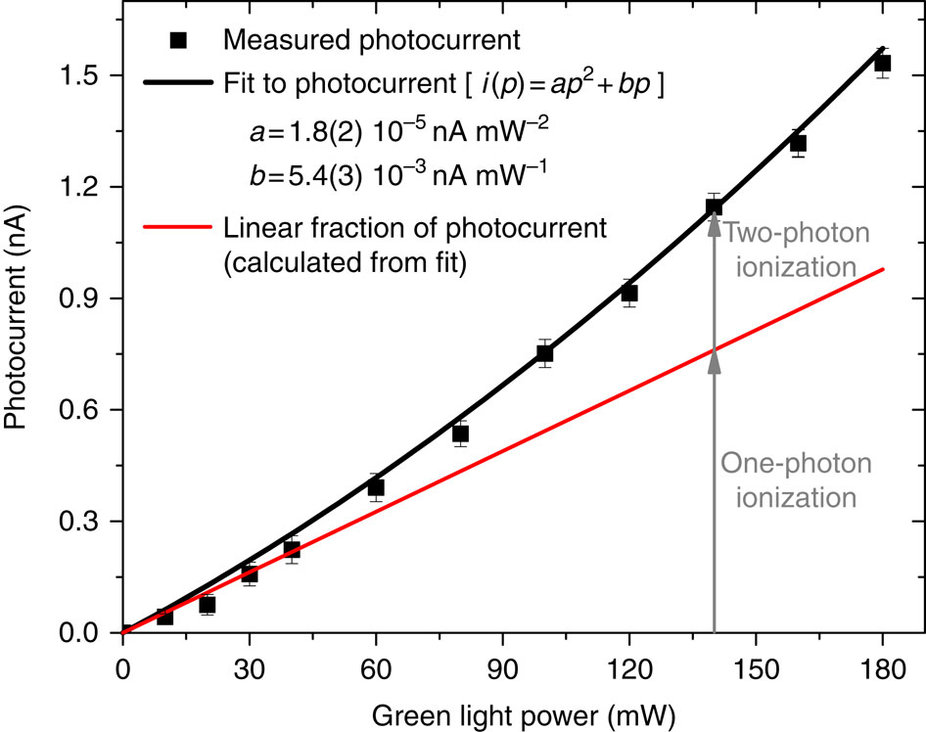
\includegraphics[width=0.45\textwidth]{Images/TwoPhotonPlot.jpg}

    E. Bourgeois, et al. Nat. Commun. 6, 8577 (2015).
\end{frame}

\begin{frame}\frametitle{Single-Photon Electroluminescence}
    \begin{block}{Ion-Microbeam Buried Electrodes}
        \centering
        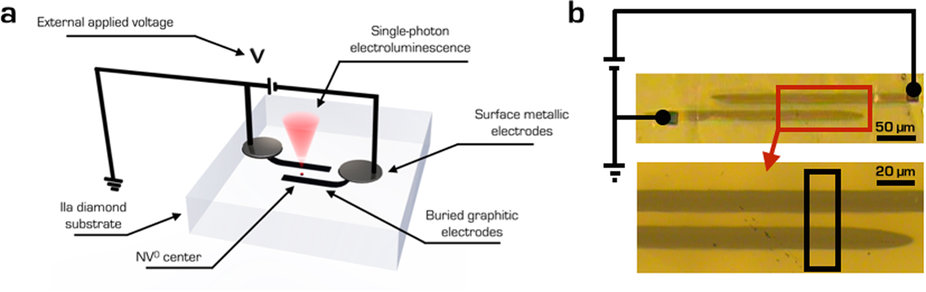
\includegraphics[width=0.95\textwidth]{Images/Electrolumin.jpg}

        J. Forneris, et al. Nat. Publ. Gr. 1 (2015).
    \end{block}
\end{frame}

\begin{frame}\frametitle{Proposed Micro-diamond Electrode Process}
    \centering
    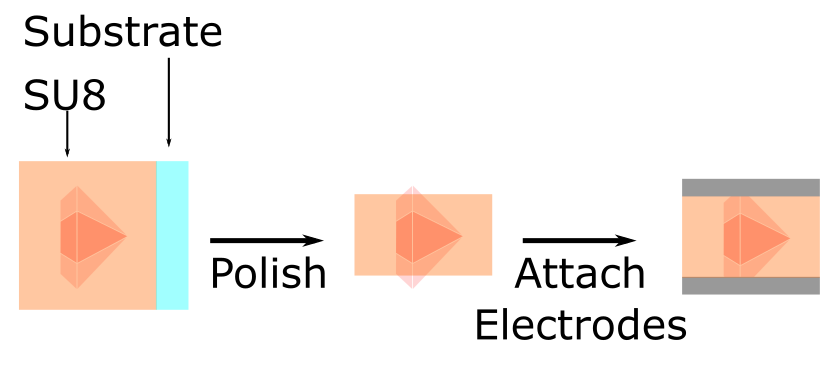
\includegraphics[width=0.95\textwidth]{Images/ElectrodeProcess.png}
\end{frame}

\begin{frame}\frametitle{Proposed Singlet State Photoionization}
    \centering
    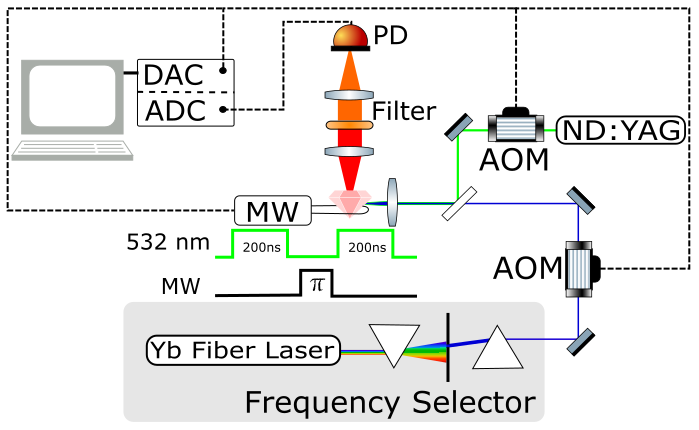
\includegraphics[width=0.95\textwidth]{Images/WP1Schematic.png}
\end{frame}

\begin{frame}\frametitle{Conclusions}
    \begin{itemize}
        \item Singlet state ionization is a single photon process.
        \item If we can ionize from the singlet state we should be able to measure a photocurrent with a linear dependence on pump power.
    \end{itemize}
\end{frame}

\end{document}

